\chapter{\label{a3-spe}SPE Fitting}

\minitoc

\section{Introduction}

Due to the multiplicative process applied to a photoelectron in both \glspl{mapmt} and \glspl{sipmt}, the resulting charge distribution is quantised according to the number of photoelectrons that were produced before the multiplication. 

If an \gls{mapmt} or \gls{sipmt} is illuminated to a very low light level (such that the photosensors perform as individual photon counters), and the resulting signal is accumulated inside a histogram, the distinct peaks corresponding to the detected number of photoelectrons are observed. The resolution of these peaks is determined by the \gls{enf}, as detailed in Section~\ref{section:enf}. This visualisation is known as the \gls{spe} spectrum, and it is a powerful tool utilised in the calibration of these photosensors.

The typical characteristics of the \gls{spe} spectrum are Gaussian peaks corresponding to each photoelectron, the height of which follow a Poisson distribution corresponding to the average illumination level that was present when taking the data.

Typically, the following features from the \gls{spe} spectra can be extracted with simple approaches:
\begin{itemize}
\item The position and width of the pedestal peak, indicating the level of electronic noise.
\item The position of the first photoelectron peak, suggesting the gain of the photosensor.
\item The average illumination from the ratio of the pedestal to single photoelectron peak.
\end{itemize}

\begin{figure}
	\centering
    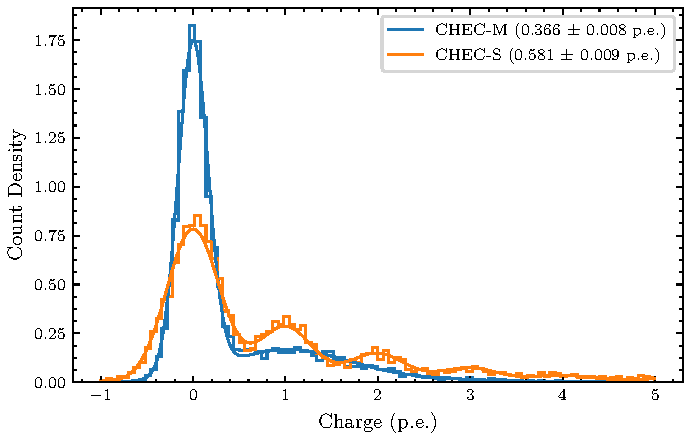
\includegraphics[width=\textwidth]{spe_checm_checs} 
	\caption[(Repeated) Comparison of SPE spectra between CHEC-M and CHEC-S.]{Repeat of Figure~\ref{fig:spe_checm_checs}. Comparison of SPE spectra between CHEC-M (MAPMT) and CHEC-S (SiPM) for a single pixel, along with their corresponding fit function. In both cases, three illuminations are simultaneously fit.} 
	\label{fig:spe_checm_checs_repeat}
\end{figure}

\begin{table}[!ht]
\centering
\begin{tabular}{ll|ll} \toprule
    Fit Parameter        &            & CHEC-M             & CHEC-S            \\ \midrule
    Average Illumination & [\si{\pe}] & 0.366 $\pm$ 0.008  & 0.581 $\pm$ 0.009 \\
    Pedestal Deviation   & [\si{\pe}] & 0.163 $\pm$ 0.001  & 0.285 $\pm$ 0.002 \\
    Gain Deviation       & [\si{\pe}] & 0.626 $\pm$ 0.009  & 0.078 $\pm$ 0.007 \\
    Optical Crosstalk    &            &                    & 0.350 $\pm$ 0.006 \\ \bottomrule
\end{tabular}
\caption{Parameter values resulting from the fit to the spectra in Figure~\ref{fig:spe_checm_checs_repeat}. The \si{1}{$\sigma$} parabolic errors obtained from the covariance matrix of the fit parameters are also quoted.}
\label{table:spe_checm_checs_repeat}
\end{table}

As is illustrated in Figure~\ref{fig:spe_checm_checs_repeat}, the resolution of the \gls{spe} peaks obtained form an \gls{mapmt} is much lower than that obtained from an \gls{sipmt}, making it difficult to characterise the \gls{spe} spectrum by eye, or by simple fits using the aforementioned features. Additionally, many factors that contribute the \gls{spe} spectrum are hard to entangle. Therefore, an analytical description, that consolidates the contributing factors of the photosensor to generate the \gls{spe} spectrum observed, is used to fit the histogram.

\section{Software}

The |extract_spe.py| script inside \pkg{CHECLabPy} allows the correct analytical function corresponding to the dataset to be chosen at runtime. It then utilises the |SpectrumFitter| class to flexibly fit $N$ datasets of different illuminations simultaneously. This simultaneous fit helps to disentangle certain parameters. In the case of the \glspl{sipmt} the optical crosstalk and average illumination are closely entangled, and a fit to a single illumination can have trouble providing accurate values. However, when increasing the average illumination, the optical crosstalk remains constant. The fit can therefore better constrain the difference each parameter contributes. Furthermore, the |extract_spe.py| script fits each pixel in parallel, considerably reducing the runtime.

\section{Multi-Anode Photomultiplier Tubes}

The behaviour of a \gls{pmt} (which extends to \glspl{mapmt}) is very well understood, and is simple to quantify. 

At an average illumination $\lambda$, there exists a probability to get either 0, 1, 2, 3...$k$ photoelectrons, defined by the Poisson distribution:
\begin{equation} \label{eq:mapm_spe_poisson}
P(k) = \me^{-\lambda} \frac{\lambda^k}{k!}.
\end{equation}

The distribution of values from Equation~\ref{eq:mapm_spe_poisson} are delta functions at each photoelectron value. This corresponds to the \gls{spe} spectrum you would measure for a perfect photosensor, with no electronic noise or \gls{enf}. 

In the case $k = 0$ (the pedestal peak), the probability to measure a charge $q$ (in \si{mV}, \si{mVns}, \si{ADC}, or \si{\pe}, depending on the calibration applied and the charge extraction approach used) is represented as a Gaussian with area $P(0)$, standard deviation $\sigma_0$ (representing the variation in electronic noise), and a mean $\mu_0$ (as the baseline of the waveforms may not be corrected):
\begin{equation} \label{eq:mapm_spe_ped}
P(q) = e^{-\lambda} \frac{1}{\sqrt{2 \pi \sigma_0^2}} e^{-\frac{(q - \mu_0)^2}{2 \sigma_0^2}}.
\end{equation}

In the case $k > 0$, the mean and the standard deviation of the Gaussian increases with $k$. Additionally, the pedestal spread is also present in the $k > 0$ peaks. Therefore, the probability to measure a charge $q$ is expressed as a Gaussian with area $P(k)$. The standard deviation $\sigma(k)$ is expressed as the quadrature sum of the two contributions:
\begin{equation}
\sigma(k) = \sqrt{\sigma_0^2 + k \sigma_1^2},
\end{equation}
where $\sigma_1$ is the standard deviation in the multiplication of a single photoelectron.
The mean $\mu(k)$ is the mean of the first photoelectron peak $\mu_1$ multiplied by $k$. This results in the expression:
\begin{equation}
P(q, k) = P(k) \frac{1}{\sqrt{2 \pi \sigma(k)^2}} e^{-\frac{(q - \mu(k))^2}{2 \sigma(k)^2}}.
\end{equation}

The sum over each distribution of $P(q)$, for each value of $k$ (I only go up to $k=10$), gives the probability of getting each value of charge $q$. Combined with a normalisation factor, this equation can then be used to fit the spectrum of an \gls{mapmt}.

\section{Silicon Photomultipliers}

The analytical description for an \gls{sipmt} is a bit more complicated. The formula we have found to work well is the one described by \textcite{Gentile2010}. It expands on the formula I have described for \glspl{mapmt} to include the \gls{sipmt} optical crosstalk and afterpulsing.

As with \glspl{mapmt}, the probability to get $k$ initial photoelectrons (i.e.\@ $k$ initially fired microcells) follows a Poisson distribution. However, to find the probability of getting a total number of fired microcells $n$, the optical crosstalk probability~$\epsilon$, must be included:
\begin{equation}
P(n) = \sum_{k=1}^n P(k) (1 - \epsilon)^k \epsilon^{n-k} \binom{n-1}{k-1}.
\end{equation}

The formula for the probability of obtaining a charge $q$ is also similar to the \gls{mapmt} case. However, two additional terms are included to account for two levels of afterpulsing, occurring at a reduced charge of $\delta_1$ and $\delta_2$ from the photoelectron peaks, each with a probability of that level of afterpulsing occurring. Due to the diminished afterpulsing probability in recent \gls{sipmt} productions (Section~\ref{section:sipmt_parameters}), we removed the second level of afterpulsing from the fit, as we already get a very small value from using the first afterpulse level in the fit.